\documentclass[a4paper, 12pt]{report}
\usepackage{fullpage}
\usepackage{graphicx}
\usepackage[indonesian]{babel}

\graphicspath{{./figures/}}


\title{
    \Huge
    {Kumpulan Write-up}\\
    \vfill
    {
\includegraphics[scale=2]{iteba.png}}
}

\author{CTF Club ITEBA\\Andrian Syah\\Kevin Antony\\Hani Kahiriyah}
\date{} % to add date use "\today" inside \date{}

\newcommand\chap[1]{%
  \chapter*{#1}%
  \addcontentsline{toc}{chapter}{#1}}

\begin{document}
\maketitle

\tableofcontents


% halaman forensik %%%%%%%%%%%%%%%%%%%%%%%%%%%%%%%%%%%%%%%%%%%%%%%%%%%%%%%%%%%%%
\newpage
\chapter*{Forensic}
\addcontentsline{toc}{chapter}{Forensic}

\section*{PNG\_or\_Not}
\addcontentsline{toc}{section}{PNG\_or\_Not}
\subsection*{Soal}
Mencari Flag yang ada pada file yang diberikan dalam bentuk file:data tanpa adanya signature file

\subsection*{Solusi}
Analisis file menggunakan utility di ubuntu yaitu : binwalk dan foremost , namun juga menggunakan Penerjemah Hex 
untuk mencari flag yang ada di dalam nya . disini menggunakan Code Editor yang ada diwindows untuk dapat mencari flag .
dan mengubah string yang ada pada flag menjadi base64 encode .

{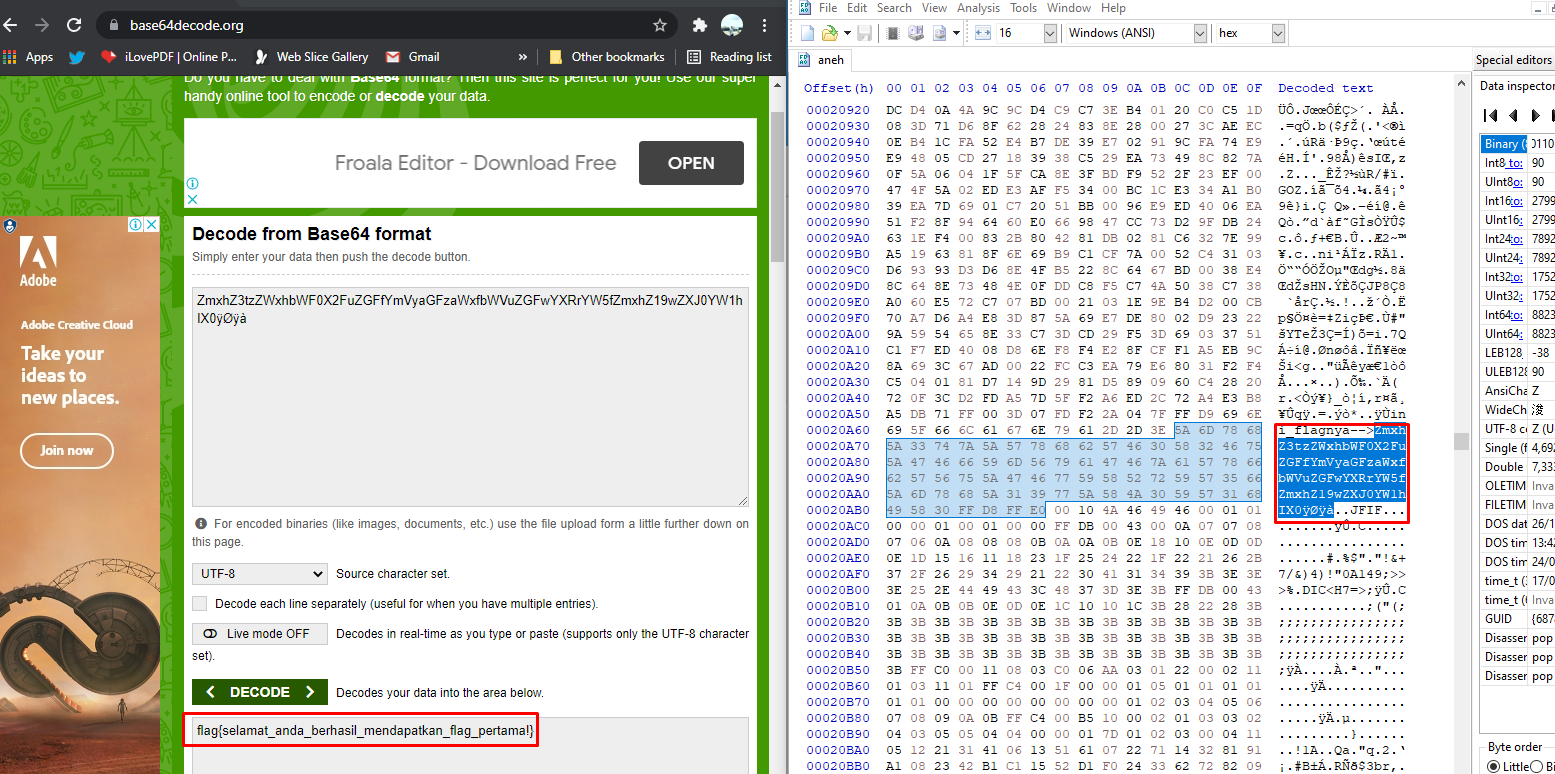
\includegraphics[scale=0.4]{pngornot.png}}

\section*{disk.img}
\addcontentsline{toc}{section}{disk.img}
\subsection*{Soal}
deskripsi Soal
\subsection*{Solusi}
deskripsi solusi

% halaman web  exploitation %%%%%%%%%%%%%%%%%%%%%%%%%%%%%%%%%%%%%%%%%%%%%%%%%%%%
\newpage
\chapter*{Web Exploitation}
\addcontentsline{toc}{chapter}{Web Exploitation}



\end{document}